% Pengaturan ukuran teks dan bentuk halaman dua sisi
\documentclass[12pt, twoside]{report}

% Pengaturan ukuran halaman dan margin
\usepackage[a4paper,top=30mm,left=30mm,right=20mm,bottom=25mm]{geometry}

% Pengaturan ukuran spasi
\usepackage[singlespacing]{setspace}

% Pengaturan caption untuk tabel
\usepackage{caption}

% Judul dokumen
\title{Proposal Tugas Akhir ITS}
\author{Musk, Elon Reeve}

% Pengaturan detail pada file PDF
\usepackage[pdfauthor={\@author},bookmarksnumbered,pdfborder={0 0 0}]{hyperref}


% Pengaturan ukuran indentasi
\setlength{\parindent}{2em}

% Package lainnya
\usepackage{changepage}
\usepackage{etoolbox} % Mengubah fungsi default

% Pengaturan jenis karakter
\usepackage[utf8]{inputenc}

\usepackage[style=ieee, backend=biber]{biblatex}
\usepackage{enumitem} % Pembuatan list
\usepackage{lipsum} % Pembuatan template kalimat
\usepackage{graphicx} % Input gambar
\usepackage{longtable} % Pembuatan tabel
\usepackage[table,xcdraw]{xcolor} % Pewarnaan tabel
\usepackage{eso-pic} % Untuk menggunakan background image di halaman
\usepackage{txfonts} % Font times
\usepackage{changepage} % Pembuatan teks kolom
\usepackage{multicol} % Pembuatan kolom ganda
\usepackage{multirow} % Pembuatan baris ganda
\usepackage{tabularx} % Untuk mengatur kolom, seperti grid pada CSS
\usepackage{wrapfig}
\usepackage{ragged2e}
\usepackage[none]{hyphenat}


\usepackage{caption} 
% Separator style
\DeclareCaptionLabelSeparator{custom}{. }
\captionsetup{
  labelsep=custom
}

% Pengaturan format daftar isi, daftar gambar, dan daftar tabel
\usepackage{tocloft}
\setlength{\cftbeforechapskip}{1.5ex}
\setlength{\cftbeforesecskip}{1.5ex}
\setlength{\cftbeforetoctitleskip}{0cm}
\setlength{\cftbeforeloftitleskip}{0cm}
\setlength{\cftbeforelottitleskip}{0cm}
\renewcommand{\cfttoctitlefont}{\hfill\Large\bfseries} % command untuk membuat heading bold dan besar
\renewcommand{\cftaftertoctitle}{\hfill}
\renewcommand{\cftloftitlefont}{\hfill\Large\bfseries}
\renewcommand{\cftafterloftitle}{\hfill}
\renewcommand{\cftlottitlefont}{\hfill\Large\bfseries}
\renewcommand{\cftafterlottitle}{\hfill}

% Definisi untuk "Hati ini sengaja dikosongkan"
\patchcmd{\cleardoublepage}{\hbox{}}{
  \thispagestyle{empty}
  \vspace*{\fill}
  \begin{center}\textit{[Halaman ini sengaja dikosongkan]}\end{center}
  \vfill}{}{}

  % Pengaturan penomoran halaman
\usepackage{fancyhdr}
\fancypagestyle{plain}{% Redefining plain page style
  \fancyhf{} %clear all header and footer fields
  \fancyfoot[C]{\thepage}
}%
\fancyhf{}
\renewcommand{\headrulewidth}{0pt}
\pagestyle{fancy}
\fancyfoot[C]{\thepage}
\patchcmd{\chapter}{plain}{fancy}{}{}
\patchcmd{\chapter}{empty}{plain}{}{}

% Pengaturan format judul bab
\usepackage{titlesec}
\renewcommand{\thesection}{\thechapter.\arabic{section}}
\titleformat{\chapter}[hang]{\centering\bfseries\Large}{BAB\ \arabic{chapter}\ }{0ex}{\vspace{0ex}\centering}
\titleformat*{\section}{\large\bfseries}
\titleformat*{\subsection}{\normalsize\bfseries}
\titlespacing{\chapter}{0ex}{0ex}{4ex}
\titlespacing{\section}{0ex}{1ex}{1ex}
\titlespacing{\subsection}{0ex}{1ex}{1ex}
\titlespacing{\subsubsection}{0ex}{1ex}{1ex}
\setcounter{secnumdepth}{3} % Untuk memberi penomoran pada \subsubsection

\counterwithin{figure}{chapter}
\counterwithin{table}{chapter}

% Mengganti figure dan table menjadi gambar dan tabel
\renewcommand{\figurename}{Gambar}
\renewcommand{\tablename}{Tabel}

% Tambahkan format tanda hubung yang benar di sini
\hyphenation{
  ro-ket
  me-ngem-bang-kan
  per-hi-tu-ngan
  ku-a-li-tas
  meng-a-wa-si
  ken-da-ra-an
  con-vo-lu-tion
  me-la-ku-kan
  me-nga-wa-si
  mes-ki-pun
}

% Menambahkan resource daftar pustaka
\addbibresource{pustaka/pustaka.bib}

% Isi keseluruhan dokumen
\begin{document}

\sloppy

% Sampul Bahasa Indonesia
\newcommand\covercontents{sampul/konten-id.tex}
\AddToShipoutPictureBG*{
  \AtPageLowerLeft{
    % Ubah nilai berikut jika posisi horizontal background tidak sesuai
    \hspace{-3.5mm}

    % Ubah nilai berikut jika posisi vertikal background tidak sesuai
    \raisebox{0mm}{
      
\includegraphics[width=\paperwidth,height=\paperheight]{sampul/gambar/sampul-luar.png}
    }
  }
}

% Menyembunyikan nomor halaman
\thispagestyle{empty}

% Pengaturan margin untuk menyesuaikan konten sampul
\newgeometry{
  top=60mm,
  left=25mm,
  right=30mm,
  bottom=25mm
}

\begin{flushleft}
  \begin{spacing}{1.5}
    % Pemilihan font sans serif
    \sffamily

    % Pemilihan warna font putih
    \color{white}

    % Pemilihan font bold
    \fontseries{bx}
    \selectfont

    \input{\covercontents}


  \end{spacing}
\end{flushleft}

\restoregeometry

\cleardoublepage


% Sampul Bahasa Indonesia
\renewcommand\covercontents{sampul/konten-id.tex}
\AddToShipoutPictureBG*{
  \AtPageLowerLeft{
    % Ubah nilai berikut jika posisi horizontal background tidak sesuai
    \hspace{-3.25mm}

    % Ubah nilai berikut jika posisi vertikal background tidak sesuai
    \raisebox{0mm}{
      
\includegraphics[width=\paperwidth,height=\paperheight]{sampul/gambar/sampul-luar-tipis.png}
    }
  }
}

% Menyembunyikan nomor halaman
\thispagestyle{empty}

% Pengaturan margin untuk menyesuaikan konten sampul
\newgeometry{
  top=70mm,
  left=30mm,
  right=30mm,
  bottom=20mm
}

\begin{flushleft}

  % Pemilihan font sans serif
  \sffamily

  % Pemilihan font bold
  \fontseries{bx}
  \selectfont
  \begin{spacing}{1.5}
    \input{\covercontents}
  \end{spacing}

\end{flushleft}

\restoregeometry

\newpage
\cleardoublepage

% Sampul Bahasa Inggris
\renewcommand\covercontents{sampul/konten-en.tex}
\AddToShipoutPictureBG*{
  \AtPageLowerLeft{
    % Ubah nilai berikut jika posisi horizontal background tidak sesuai
    \hspace{-3.25mm}

    % Ubah nilai berikut jika posisi vertikal background tidak sesuai
    \raisebox{0mm}{
      
\includegraphics[width=\paperwidth,height=\paperheight]{sampul/gambar/sampul-luar-tipis.png}
    }
  }
}

% Menyembunyikan nomor halaman
\thispagestyle{empty}

% Pengaturan margin untuk menyesuaikan konten sampul
\newgeometry{
  top=70mm,
  left=30mm,
  right=30mm,
  bottom=20mm
}

\begin{flushleft}

  % Pemilihan font sans serif
  \sffamily

  % Pemilihan font bold
  \fontseries{bx}
  \selectfont
  \begin{spacing}{1.5}
    \input{\covercontents}
  \end{spacing}

\end{flushleft}

\restoregeometry

\newpage
\cleardoublepage

% Nomor halaman pembuka dimulai dari sini
\pagenumbering{roman}

% Atur ulang penomoran halaman
\setcounter{page}{1}

% Lembar pengesahan
\begin{center}
  \large
  \textbf{LEMBAR PENGESAHAN}
\end{center}

\vspace{4mm}

% % Menyembunyikan nomor halaman
% \thispagestyle{empty}

\begin{center}
  % Ubah kalimat berikut dengan judul tugas akhir
  \textbf{
    REIDENTIFIKASI KENDARAAN MENGGUNAKAN \emph{CONVOLUTIONAL NEURAL NETWORK} (CNN)
    PADA CITRA \emph{UNMANNED AERIAL VEHICLE} (UAV)
  }
\end{center}

\begingroup
% Pemilihan font ukuran small
\small

\begin{center}
  % Ubah kalimat berikut dengan pernyataan untuk lembar pengesahan
  \textbf{TUGAS AKHIR} \\
  Diajukan untuk memenuhi salah satu syarat memperoleh gelar
  Sarjana Teknik pada
  Program Studi S-1 Teknik Komputer \\
  Departemen Teknik Komputer \\
  Fakultas Teknologi Elektro dan Informatika Cerdas \\
  Institut Teknologi Sepuluh Nopember
\end{center}

\begin{center}
  % Ubah kalimat berikut dengan nama dan NRP mahasiswa
  Oleh: \textbf{Wildan Shafa Diandra} \\
  NRP. 07211940000049
\end{center}

\begin{center}
  Disetujui oleh Tim Penguji Tugas Akhir:
\end{center}

\begingroup
% Menghilangkan padding
\setlength{\tabcolsep}{0pt}

\noindent
\begin{tabularx}{\textwidth}{X c}
  % Ubah kalimat-kalimat berikut dengan nama dan NIP dosen pembimbing pertama
  Reza Fuad Rachmadi, S.T., M.T., Ph.D &                 \\
  NIP: 198504032012121001              & (Pembimbing)    \\
                                       &                 \\
                                       &                 \\
  % Ubah kalimat-kalimat berikut dengan nama dan NIP dosen pembimbing kedua
  Dr. I Ketut Eddy Purnama, S.T., M.T. &                 \\
  NIP: 196907301995121001              & (Ko-Pembimbing) \\
                                       &                 \\
                                       &                 \\
  % Ubah kalimat-kalimat berikut dengan nama dan NIP dosen penguji pertama
  Penguji I                            &                 \\
  NIP:                                 & (Penguji I)     \\
                                       &                 \\
                                       &                 \\
  % Ubah kalimat-kalimat berikut dengan nama dan NIP dosen penguji kedua
  Penguji II                           &                 \\
  NIP:                                 & (Penguji II)    \\
                                       &                 \\
                                       &                 \\
  % Ubah kalimat-kalimat berikut dengan nama dan NIP dosen penguji ketiga
  Penguji III                          &                 \\
  NIP:                                 & (Penguji III)   \\
\end{tabularx}
\endgroup

\vspace{2ex}

\begin{center}
  % Ubah kalimat berikut dengan jabatan kepala departemen
  Mengetahui, \\
  Kepala Departemen Teknik Dirgantara FTD - ITS \\

  \vspace{10ex}

  % Ubah kalimat-kalimat berikut dengan nama dan NIP kepala departemen
  \underline{Dr. Leonardo Da Vinci, S.T., M.T.} \\
  NIP. 14520415 151905 1 001
\end{center}

\vfill

\begin{center}
  % Ubah text dibawah menjadi tempat dan tanggal
  \textbf{SURABAYA} \\
  \textbf{Desember, 2022}
\end{center}
\endgroup

\newpage
\cleardoublepage

% Lembar pengesahan
\begin{center}
  \large
  \textbf{APPROVAL SHEET}
\end{center}

% Menyembunyikan nomor halaman
\thispagestyle{empty}

\begin{center}
  % Ubah kalimat berikut dengan judul tugas akhir
  \textbf{
    VEHICLE REIDENTIFICATION USING CONVOLUTIONAL NEURAL NETWORK (CNN)
    ON UNMANNED AERIAL VEHICLE (UAV) IMAGES}
\end{center}

\begingroup
% Pemilihan font ukuran small
\small

\begin{center}
  % Ubah kalimat berikut dengan pernyataan untuk lembar pengesahan
  \textbf{FINAL PROJECT} \\
  Submitted to fulfill one of the requirements for obtaining a degree
  Bachelor of Engineering at
  Undergraduate Study Program of Computer Engineering \\
  Department of Computer Engineering \\
  Faculty of Intelligent Electrical and Informatics Technology \\
  Sepuluh Nopember Institute of Technology
\end{center}

\begin{center}
  % Ubah kalimat berikut dengan nama dan NRP mahasiswa
  By: \textbf{Wildan Shafa Diandra} \\
  NRP. 07211940000049
\end{center}

\begin{center}
  Approved by Final Project Proposal Examiner Team:
\end{center}

\begingroup
% Menghilangkan padding
\setlength{\tabcolsep}{0pt}

\noindent
\begin{tabularx}{\textwidth}{X c}
  % Ubah kalimat-kalimat berikut dengan nama dan NIP dosen pembimbing pertama
  Reza Fuad Rachmadi, S.T., M.T., Ph.D &                \\
  NIP: 198504032012121001              & (Advisor)      \\
                                       &                \\
                                       &                \\
  % Ubah kalimat-kalimat berikut dengan nama dan NIP dosen pembimbing kedua
  Dr. I Ketut Eddy Purnama, S.T., M.T. &                \\
  NIP: 196907301995121001              & (Co-Advisor)   \\
                                       &                \\
                                       &                \\
  % Ubah kalimat-kalimat berikut dengan nama dan NIP dosen penguji pertama
  Penguji I                            &                \\
  NIP:                                 & (Examiner I)   \\
                                       &                \\
                                       &                \\
  % Ubah kalimat-kalimat berikut dengan nama dan NIP dosen penguji kedua
  Penguji II                           &                \\
  NIP:                                 & (Examiner II)  \\
                                       &                \\
                                       &                \\
  % Ubah kalimat-kalimat berikut dengan nama dan NIP dosen penguji ketiga
  Penguji III                          &                \\
  NIP:                                 & (Examiner III) \\
\end{tabularx}
\endgroup

\vspace{2ex}

\begin{center}
  % Ubah kalimat berikut dengan jabatan kepala departemen
  Acknowledged, \\
  Head of Computer Engineering Department\\

  \vspace{10ex}

  % Ubah kalimat-kalimat berikut dengan nama dan NIP kepala departemen
  \underline{Dr. Supeno Mardi Susiki Nugroho, S.T., M.T.} \\
  NIP. 19700031319951210001
\end{center}

\vfill

\begin{center}
  % Ubah text dibawah menjadi tempat dan tanggal
  \textbf{SURABAYA} \\
  \textbf{December, 2022}
\end{center}
\endgroup


\newpage
\cleardoublepage

% Lembar pernyataan orisinalitas
\begin{center}
  \large
  \textbf{PERNYATAAN ORISINALITAS}
\end{center}

% Menyembunyikan nomor halaman
\thispagestyle{empty}

\vspace{2ex}

\noindent
Yang bertanda tangan di bawah ini:

\vspace{2ex}

\begin{adjustwidth}{0.5cm}{}
  \begin{tabular}{lcp{0.5\linewidth}}

    % Ubah kalimat-kalimat berikut sesuai dengan nama dan NRP mahasiswa
    Nama Mahasiswa/NRP & : & Wildan Shafa Diandra/07211940000049     \\

    % Ubah kalimat berikut sesuai dengan semester pengajuan proposal
    Departemen         & : & Teknik Komputer                         \\

    % Ubah kalimat-kalimat berikut sesuai dengan nama-nama dosen pembimbing
    Dosen Pembimbing   & : & 1. Reza Fuad Rachmadi, S.T., M.T., Ph.D \\
                       &   & 2. Dr. I Ketut Eddy Purnama, S.T., M.T. \\                                                        \\
  \end{tabular}
\end{adjustwidth}

% Ubah paragraf-paragraf berikut sesuai dengan yang ingin diisi pada pernyataan keaslian

dengan ini menyatakan bahwa Tugas Akhir dengan judul “Reidentifikasi Kendaraan Menggunakan Convolutional Neural Network (CNN) Pada Citra Unmanned Aerial Vehicle (UAV)” adalah hasil karya sendiri, bersifat orisinal, dan ditulis dengan mengikuti kaidah penulisan ilmiah.

Bilamana di kemudian hari ditemukan ketidaksesuaian dengan pernyataan ini, maka saya bersedia menerima sanksi sesuai dengan ketentuan yang berlaku di Institut Teknologi Sepuluh Nopember.

\vspace{2ex}

\begin{flushright}
  Surabaya, Juli 2023
\end{flushright}

\vspace{2ex}

\begin{center}

  \begin{multicols}{2}

    Mengetahui, \\
    Dosen Pembimbing
    \vspace{12ex}

    % Ubah kalimat-kalimat berikut sesuai dengan nama dan NIP dosen pembimbing pertama
    \underline{Reza Fuad Rachmadi, S.T., M.T., Ph.D} \\
    NIP. 198504032012121001

    \columnbreak

    \hfill \break
    Mahasiswa
    \vspace{12ex}

    % Ubah kalimat-kalimat berikut sesuai dengan nama dan NIP dosen pembimbing kedua
    \underline{Wildan Shafa Diandra} \\
    NRP. 07211940000049

  \end{multicols}

\end{center}
\newpage
\cleardoublepage

% Lembar pernyataan orisinalitas
\begin{center}
  \large
  \textbf{STATEMENT OF ORIGINALITY}
\end{center}

% Menyembunyikan nomor halaman
\thispagestyle{empty}

\vspace{2ex}

\noindent
The undersigned below:

\vspace{2ex}

\begin{adjustwidth}{0.5cm}{}
  \begin{tabular}{lcp{0.5\linewidth}}

    % Ubah kalimat-kalimat berikut sesuai dengan nama dan NRP mahasiswa
    Name of Student/NRP & : & Wildan Shafa Diandra/07211940000049     \\

    % Ubah kalimat berikut sesuai dengan semester pengajuan proposal
    Departmen           & : & Computer Engineering                    \\

    % Ubah kalimat-kalimat berikut sesuai dengan nama-nama dosen pembimbing
    Advisor             & : & 1. Reza Fuad Rachmadi, S.T., M.T., Ph.D \\
                        &   & 2. Dr. I Ketut Eddy Purnama, S.T., M.T. \\                                                        \\
  \end{tabular}
\end{adjustwidth}

% Ubah paragraf-paragraf berikut sesuai dengan yang ingin diisi pada pernyataan keaslian

hereby declare that the Final Project with the title of ”Vehicle Reidentification Using Convolutional Neural Network (CNN) On Unmanned Aerial Vehicle (UAV) Images” is the result of my own work, is original, and is written by following the rules of scientific writing.

If in the future there is a discrepancy with this statement, then I am willing to accept sanctions in accordance with the provisions that apply at Institut Teknologi Sepuluh Nopember.

\vspace{2ex}

\begin{flushright}
  Surabaya, July 2023
\end{flushright}

\vspace{2ex}

\begin{center}

  \begin{multicols}{2}

    Acknowledged, \\
    Advisor
    \vspace{12ex}

    % Ubah kalimat-kalimat berikut sesuai dengan nama dan NIP dosen pembimbing pertama
    \underline{Reza Fuad Rachmadi, S.T., M.T., Ph.D} \\
    NIP. 198504032012121001

    \columnbreak

    \hfill \break
    Student
    \vspace{12ex}

    % Ubah kalimat-kalimat berikut sesuai dengan nama dan NIP dosen pembimbing kedua
    \underline{Wildan Shafa Diandra} \\
    NRP. 07211940000049

  \end{multicols}

\end{center}
\newpage
\cleardoublepage

% Abstrak
\addcontentsline{toc}{chapter}{ABSTRAK}

\begin{center}
  \large
  \textbf{ABSTRAK}
\end{center}

\vspace{4mm}

\begin{center}
  \textbf{
    REIDENTIFIKASI KENDARAAN MENGGUNAKAN \emph{CONVOLUTIONAL NEURAL NETWORK} (CNN)
    PADA CITRA \emph{UNMANNED AERIAL VEHICLE} (UAV)
  }
\end{center}

% % Menyembunyikan nomor halaman
% \thispagestyle{empty}

\begin{flushleft}
  \setlength{\tabcolsep}{0pt}
  \bfseries
  \begin{tabular}{ll@{\hspace{6pt}}l}
    Nama Mahasiswa / NRP & : & Wildan Shafa Diandra / 07211940000049   \\
    Departemen           & : & Teknik Komputer FTEIC - ITS             \\
    Dosen Pembimbing     & : & 1. Reza Fuad Rachmadi, S.T., M.T., Ph.D \\
                         &   & 2. Dr. I Ketut Eddy Purnama, S.T., M.T. \\
  \end{tabular}
  \vspace{4ex}
\end{flushleft}
\textbf{Abstrak}

% Isi Abstrak
Beberapa tahun terakhir jumlah kendaraan bermotor di Indonesia terus meningkat. Sejumlah besar kamera pengintai digunakan di sudut-sudut jalan maupun persimpangan untuk membantu proses pemantauan lalu lintas. Sistem pemantauan tersebut sebagian besar berbasis video real-time dan masih membutuhkan manusia untuk mengawasinya sehingga masih kurang efektif. Selain itu, penggunaan kamera pengintai juga kurang efektif apabila digunakan untuk mengawasi banyak lokasi. Satu buah kamera pengintai hanya bisa digunakan untuk mengawasi 1 titik lokasi. Saat ini penelitian mengenai system reidentifikasi mobil berbasis CNN mulai banyak dikembangkan. Sistem reidentifikasi mobil dapat membantu proses pemantauan lalu lintas khususnya dalam memantau, melacak, maupun mencari mobil. Pada saat yang sama, pemanfaatan Unmanned Aerial Vehicles (UAV) mulai banyak digunakan di berbagai sektor kehidupan, salah satunya di bidang visi komputer. Pada penelitian ini, penulis ingin membuat model CNN yang dapat melakukan reidentifikasi mobil. Dataset yang akan digunakan pada penelitian ini diambil menggunakan UAV. Penulis berharap dengan adanya penelitian ini, penelitian tentang teknologi identifikasi ulang mobil yang memanfaatkan UAV akan lebih banyak dipelajari oleh para peneliti. Penulis juga berharap sistem reidentifikasi mobil dapat diimplementasikan pada sistem pemantauan lalu lintas sehingga memudahkan staf yang bertugas.

\vspace{2ex}
\noindent
\textbf{Kata Kunci: \emph{Convolutional Neural Network, Reidentifikasi Mobil, Unmanned Aerial Vehicle}}
\newpage
\cleardoublepage

\addcontentsline{toc}{chapter}{ABSTRACT}

\begin{center}
  \large
  \textbf{ABSTRACT}
\end{center}

\vspace{4mm}

\begin{center}
  \textbf{
    VEHICLE REIDENTIFICATION USING CONVOLUTIONAL NEURAL NETWORK (CNN)
    ON UNMANNED AERIAL VEHICLE (UAV) IMAGES
  }
\end{center}

% % Menyembunyikan nomor halaman
% \thispagestyle{empty}

\begin{flushleft}
  \setlength{\tabcolsep}{0pt}
  \bfseries
  \begin{tabular}{lc@{\hspace{6pt}}l}
    Student Name / NRP & : & Wildan Shafa Diandra/ 07211940000049    \\
    Department         & : & Computer Engineering ELECTICS - ITS     \\
    Advisor            & : & 1. Reza Fuad Rachmadi, S.T., M.T., Ph.D \\
                       &   & 2. Dr. I Ketut Eddy Purnama, S.T., M.T. \\
  \end{tabular}
  \vspace{4ex}
\end{flushleft}
\textbf{Abstract}

% Isi Abstrak
In recent years the number of motor vehicle in Indonesia has continued to increase. A large number of surveillance cameras are used on street corners and intersections to assist in the traffic monitoring process. The monitoring system is mostly based on real-time video and still requires humans to monitor it, so it is still ineffective. In addition, the use of surveillance cameras is also less effective when used to monitor multiple locations. One surveillance camera can only be used to monitor 1 location point. Currently, studies on CNN-based car re-identification systems have begun to be developed more. A car re-identification system can help the traffic monitoring process, especially in monitoring, tracking, and finding cars. At the same time, the utilization of Unmanned Aerial Vehicles (UAV) has begun to be widely used in various sectors of life, one of which is in the field of computer vision. In this study, the author wanted to create a CNN model that could carry out a car re-identification process. The dataset that will be used in this study was taken using UAV. The author hopes that with this study, studies on car re-identification system that utilizes UAVs will be studied more by many researchers. The author also hopes that the car re-identification system can be implemented in a traffic monitoring system to make it easier for the staff in charge.

\vspace{2ex}
\noindent
\textbf{Keywords: \emph{Convolutional Neural Network, Car Re-identification, Unmanned Aerial Vehicle}}
\newpage
\cleardoublepage

\begin{spacing}{1.5}
  % Daftar isi
  \renewcommand*\contentsname{DAFTAR ISI}
  \addcontentsline{toc}{chapter}{\contentsname}
  \tableofcontents
  \newpage
  \cleardoublepage

  % Daftar gambar
  \renewcommand*\listfigurename{DAFTAR GAMBAR}
  \addcontentsline{toc}{chapter}{\listfigurename}
  \listoffigures
  \newpage
  \cleardoublepage

  % Daftar tabel
  \renewcommand*\listtablename{DAFTAR TABEL}
  \addcontentsline{toc}{chapter}{\listtablename}
  \listoftables
  \newpage
  \cleardoublepage
\end{spacing}

% Nomor halaman isi dimulai dari sini
\pagenumbering{arabic}

% Konten pendahuluan
\chapter{PENDAHULUAN}
\label{chap:pendahuluan}

\section{Latar Belakang}
\label{sec:latarbelakang}

Jumlah kendaraan bermotor di Indonesia mencapai lebih dari 136 juta unit pada tahun 2020. Data itu terangkum dalam catatan Badan Pusat Statistik (BPS) \cite{DataKendaraanBermotor}. Jumlah kendaraan naik sekitar tujuh persen sejak tahun 2018. Pada tahun 2020, jumlah kendaraan naik bertambah 2.520.439 unit atau meningkat 1,8 persen menjadi 136.137.451 unit dari tahun sebelumnya sebanyak 133.617.012 unit. Jumlah kendaraan di tahun 2019 naik 5,6 persen dari tahun 2018 sejumlah 126.508.776 unit. Kenaikan jumlah kendaraan tersebut menjadi tantangan tersendiri khususnya bagi pihak kepolisian Indonesia dalam menciptakan kondisi lalu lintas yang aman dan nyaman.

Sejumlah besar kamera pengintai digunakan di sudut-sudut jalan maupun persimpangan untuk pemantauan lalu lintas. Adanya kamera pengintai memudahkan staf yang bertugas dalam melakukan pemantauan tersebut. Saat ini, sistem pemantauan lalu lintas sebagian besar berbasis video real-time dan masih membutuhkan manusia untuk mengawasinya. Banyaknya data vidio yang harus dipantau maupun kualitas vidio yang kurang baik akan menyulitkan staf pengawas yang bertugas, sehingga proses pemantauan lalu lintas akan terhambat. Selain itu, penggunaan kamera pengintai juga kurang efektif apabila digunakan untuk mengawasi banyak lokasi. Satu buah kamera pengintai hanya bisa digunakan untuk mengawasi 1 titik lokasi.

Dalam beberapa tahun terakhir, model \emph{deep learning} berbasis \emph{Convolutional Neural Network} (CNN) telah mencapai kesuksesan besar di bidang visi komputer. Salah satunya adalah sistem reidentifikasi mobil. Dengan memanfaatkan \emph{deep learning}, proses pelacakan mobil dapat dilakukan secara otomatis. Teknologi reidentifikasi mobil bekerja dengan cara mengambil citra mobil di beberapa kamera di bawah perspektif pemantauan tertentu. Citra tersebut lalu diproses oleh sistem yang mengekstrak fitur dan mencocokkannya untuk menentukan apakah citra mobil yang diberikan adalah mobil yang sama. Pada saat yang sama, perkembangan \emph{Unmanned Aerial Vehicle} juga semakin pesat. \emph{Unmanned Aerial Vehicle} atau yang selanjutnya disebut UAV merupakan jenis pesawat terbang yang dikendalikan alat sistem kendali jarak jauh lewat gelombang radio. Pemanfaatan UAV telah memberi banyak manfaat di berbagai sektor. Namun, sistem reidentifikasi mobil berbasis UAV masih jarang dipelajari. Dengan memanfaatkan UAV, pemantauan banyak lokasi akan lebih efektif. Satu buah UAV dapat digunakan untuk memantau banyak lokasi, dibandingkan dengan kamera pengintai yang membutuhkan pemasangan banyak kamera di beberapa titik lokasi pemantauan.

Pada penelitian ini, penulis ingin membuat model CNN yang dapat melakukan reidentifikasi mobil. Dataset yang akan digunakan pada penelitian ini diambil menggunakan UAV. Penulis berharap dengan adanya penelitian ini, penelitian tentang teknologi reidentifikasi mobil dengan memanfaatkan UAV akan lebih banyak dipelajari oleh para peneliti. Penulis juga berharap teknologi reidentifikasi mobil dapat memudahkan staf yang bertugas dalam pemantauan lalu lintas khususnya dalam memantau, melacak, maupun mencari kendaraan.

\section{Permasalahan}
\label{sec:permasalahan}

Berdasarkan hal yang telah dipaparkan di latar belakang, ditarik suatu permasalahan untuk judul ini yaitu sistem pengawasan berbasis video yang masih melibatkan pengawasan manusia secara manual masih kurang efektif. Banyaknya data vidio yang harus dipantau maupun kualitas vidio yang kurang baik akan menyulitkan staf pengawas yang bertugas, sehingga proses pemantauan lalu lintas khususnya dalam memantau, melacak, maupun mencari kendaraan akan terhambat. Selain itu, penggunaan kamera pengintai juga kurang efektif apabila digunakan untuk mengawasi banyak lokasi. Satu buah kamera pengintai hanya bisa digunakan untuk mengawasi 1 titik lokasi.

\section{Batasan Masalah}
\label{sec:batasanmasalah}

Batasan-batasan permasalahan yang diangkat pada penelitian ini adalah:
\begin{enumerate}[nolistsep]
    \item Penulis hanya mengembangkan model yang dapat melakukan reidentifikasi mobil. Model yang dibuat tidak diaplikasikan kepada sensor kamera.
    \item Model reidentifikasi dibuat menggunakan metode \emph{Convolutional Neural Network}.
    \item Dataset yang digunakan pada penelitian ini adalah dataset Vehicle Re-identification for Aerial Image (VRAI).
\end{enumerate}

\section{Tujuan}
\label{sec:Tujuan}

Tujuan dari penelitian ini adalah untuk menghasilkan model \emph{deep learning} yang dapat melakukan reidentifikasi mobil berbasis \emph{Convolutional Neural Network} (CNN). Model reidentifikasi dibuat dengan dataset yang menggunakan \textit{Unmanned Aerial Vehicle} (UAV) sebagai alat pengambil citra.

\section{Manfaat}
\label{sec:Manfaat}

Manfaat dari penelitian ini yaitu model reidentifikasi mobil dapat diimplementasikan pada sistem pemantauan lalu lintas sehingga bisa menjadi solusi permasalahan pada pemantauan lalu lintas.  Sistem reidentifikasi mobil diharapkan dapat mempermudah proses pemantauan lalu lintas khususnya dalam memantau, melacak, maupun mencari kendaraan. Selain itu, penggunaan \emph{Unmanned Aerial Vehicle} (UAV) juga memberi manfaat apabila diimplementasikan pada sistem pemantauan. Pemantauan banyak lokasi akan lebih efektif, sebagai contoh satu buah \emph{Unmanned Aerial Vehicle} (UAV) dapat digunakan untuk memantau banyak lokasi.

\newpage
\cleardoublepage

% Konten tinjauan pustaka
\chapter{TINJAUAN PUSTAKA}

% Ubah konten-konten berikut sesuai dengan isi dari tinjauan pustaka
\section{Hasil Penelitian Terdahulu}

\subsection{\emph{Vehicle Re-Identification System Based on Appearance Features}}
Pada tahun 2021, Dawei Xu bersama lima rekannya membuat penelitian yang berjudul "Vehicle Re-Identification System Based on Appearance Features" \cite{Xu2022}. Pada penelitian tersebut, Dawei Xu bersama lima rekannya mengusulkan metode re-identifikasi kendaraan dengan ekstrasi fitur jaringan multicabang dan fitur pengambilan dua tahap. Pengambilan dua tahap tersebut diantaranya adalah menambahkan parameter karakteristik dan penampilan kendaraan termasuk warna dan model kendaraan. Adapun dataset yang digunakan pada penelitian tersebut adalah Veri-776 dan VehicleID. Setelah melakukan penelitian menggunakan dataset dan algoritma yang sudah dibuat, mAP meningkat sebesar 2,43\% dan 2,7\% pada dua dataset yang digunakan, Rank-1 meningkat sebesar 1,85\% dan 2,9\%, dan Rank-5 meningkat sebesar 0,84\% dan 0,8\%.

\subsection{\emph{Vehicle Re-identification in Aerial Imagery : Dataset and Approach}}
Berdasarkan paper yang berjudul ”Vehicle Re-identification in Aerial Imagery: Dataset and Approach”, Peng Wang bersama lima rekannya membuat dataset untuk reidentifikasi kendaraan dengan mengaplikasikan \emph{Unmanned Aerial Vehicle} (UAV) sebagai alat pengambil citra \cite{Wang2019vehicle}. Pengaplikasian UAV telah menarik banyak perhatian baik dari sektor industri maupun akademisi. Namun, identifikasi ulang kendaraan berbasis UAV masih jarang dipelajari, meskipun memiliki banyak potensi seperti pelacakan jangka panjang, pengambilan objek visual, dan lain lain. Salah satu alasannya adalah kurangnya dataset terkait yang tersedia untuk umum. Oleh karena itu, Peng Wang bersama lima rekannya mengumpulkan dan merilis dataset VRAI (Vehicle Re-identification in Aerial Imagery) yang terdiri dari 137.613 gambar dari 13.022 sampel kendaraan.

\section{Dasar Teori}

\subsection{Reidentifikasi Mobil}

Pada dunia visi komputer, reidentifikasi adalah proses mencocokkan dua atau lebih citra suatu obyek berdasarkan identitasnya. sistem reidentifikasi yang umum dipelajari oleh para peniliti biasanya adalah sistem reidentifikasi orang dan mobil. Sebagai contoh pada sistem reidentifikasi mobil, identitas yang dicocokkan adalah warna mobil, model mobil, bumper, bentuk atap, velg ban, dan lain-lain. Dengan memanfaatkan visi komputer, proses reidentifikasi mobil dapat dilakukan secara otomatis. Sistem reidentifikas mobil bekerja dengan cara mengambil citra mobil di beberapa kamera di bawah perspektif pemantauan tertentu. Citra tersebut lalu diproses oleh sistem yang mengekstrak fitur dan mencocokkannya untuk menentukan apakah citra mobil yang diberikan adalah mobil yang sama.

\subsection{\emph{Unmanned Aerial Vehicle}}

\emph{Unmanned Aerial Vehicle} (UAV) merupakan jenis pesawat terbang yang dikendalikan alat sistem kendali jarak jauh lewat gelombang radio. \emph{Unmanned Aerial Vehicle} (UAV) merupakan sistem tanpa awak (\emph{Unmanned System}) yaitu sistem berbasis elektro mekanik yang dapat melakukan misimisi terprogram dengan karakteristik sebuah mesin terbang yang berfungsi dengan kendali jarak jauh oleh pilot atau mampu mengendalikan dirinya sendiri, menggunakan hukum aerodinamika untuk mengangkat dirinya sendiri \cite{UAV1}. \emph{Unmanned Aerial Vehicle} (UAV) mempunyai berbagai macam jenis ukuran, bentuk, dan fungsi \cite{UAV2}. Bahan material dari \emph{Unmanned Aerial Vehicle} (UAV) terbuat dari bahan yang ringan, sehingga bisa terbang dengan cepat dan terbang pada ketinggian yang rendah maupun ketinggian tertentu. \emph{Unmanned Aerial Vehicle} (UAV) sendiri memiliki kamera, infra merah, GPS, sensor, dan alat pendukung lainnya.

Saat ini masyarakat luas sudah mulai memanfaatkan \emph{Unmanned Aerial Vehicle} (UAV) untuk urusan hobi maupun militer. Salah satu contohnya adalah di dunia fotografi dan vidiografi. Para pegiat fotografi dan vidiografi profesional biasanya memiliki \emph{Unmanned Aerial Vehicle} (UAV) yang berukuran kecil dan ringan untuk memotret dan merekam objek dari ketinggian. Hal tersebut juga dilakukan oleh para peneliti khususnya di bidang visi komputer. Pemanfaatan \emph{Unmanned Aerial Vehicle} (UAV) oleh para peneliti digunakan sebagai alat pengambil citra untuk mebuat sebuah dataset. \emph{Unmanned Aerial Vehicle} (UAV) dapat menjangkau lokasi-lokasi yang sulit terjangkau oleh manusia. Selain itu, sudut tangkap kamera juga akan lebih variatif dengan memanfaatkan \emph{Unmanned Aerial Vehicle} (UAV).

\subsection{\emph{Deep Learning}}

\begin{figure} [ht] \centering
  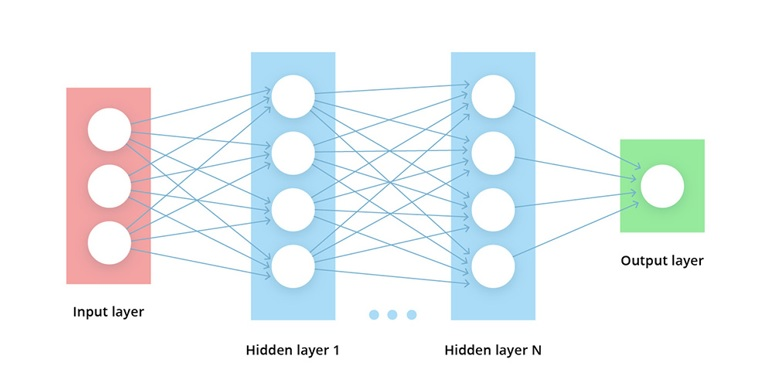
\includegraphics[scale=0.75]{gambar/deep-learning.jpg}
  \caption{\emph{Deep Learning 4 Layer} \cite{GambarDeepLearning}}
  \label{fig:DeepLearning4Layer}
\end{figure}

\emph{Deep learning} merupakan salah satu cabang dari \emph{machine learning}. \emph{Deep learning} juga merupakan salah satu algoritma dari \emph{Artificial Neural Network} yang terinspirasi dari sistem otak manusia. Algoritma pada \emph{deep learning} mempunyai kemampuan yang unik, yaitu dapat mengekstraksi fitur secara otomatis. Lapisan tersembunyi (\emph{hidden layer}) pada \emph{deep learning} lebih banyak daripada \emph{Artificial Neural Network}, sehingga pada \emph{Artificial Neural Network} membutuhkan lebih banyak informasi tentang data masukan untuk menentukan model yang cocok. Berbeda dengan \emph{deep learning} yang tidak membutuhkan informasi apapun terhadap data yang akan dipelajarinya karena secara mandiri dapat memilih model yang optimal. Beberapa contoh dari \emph{deep learning} adalah \emph{Deep Neural Network} (DNN), \emph{Recurrent Neural Network} (RNN), dan \emph{Convolutional Neural Network} (CNN). \cite{DeepLearningJWGPutra}

\subsection{\emph{Convolutional Neural Network}}

\emph{Convolutional Neural Network} (CNN) adalah salah satu jenis \emph{neural network} yang biasa digunakan pada data citra. CNN bisa digunakan untuk mendeteksi dan mengenali objek pada sebuah citra \cite{CNNQolbiyatulLina}. Secara garis besar CNN tidak jauh beda dengan \emph{neural network} lainnya. CNN terdiri dari neuron yang memiliki \emph{weight, bias} dan \emph{activation function}. \emph{Convolutional layer} juga terdiri dari neuron yang tersusun sedemikian rupa sehingga membentuk sebuah filter dengan panjang dan tinggi (\emph{pixels}).

\begin{figure} [ht] \centering
  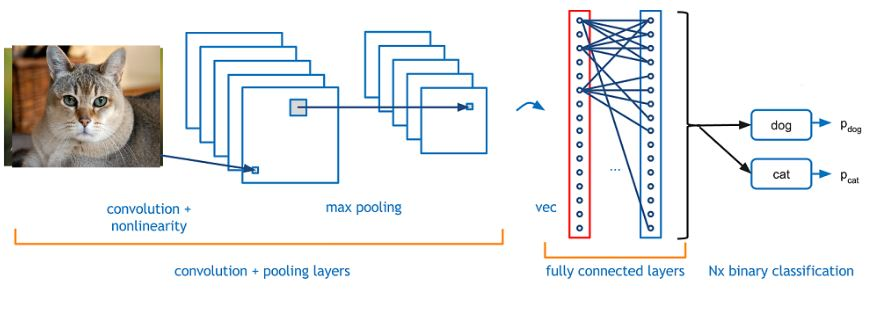
\includegraphics[scale=0.75]{gambar/cnn.jpg}
  \caption{\emph{Convolutional Neural Network} \cite{GambarCNN}}
  \label{fig:ConvolutionalNeuralNetwork}
\end{figure}

Seperti pada gambar \ref{fig:ConvolutionalNeuralNetwork}, CNN terbagi menjadi 3 \emph{layer} utama. \emph{Layer} pertama adalah \emph{convolution layer}, yang kedua adalah \emph{pooling layers}, dan terakhir adalah \emph{fully connected layers}. Berbagai jenis \emph{layer} tersebut mempunyai peran yang berbeda. \emph{Convolutional layer} digunakan untuk mengekstrasi fitur data yang akan digunakan untuk \emph{training}. Selanjutnya \emph{pooling layer} digunakan untuk membuat \emph{filter} baru berdasarkan aturan yang diinginkan (biasanya antara membuat \emph{filter} dari nilai maksimal atau membuat \emph{filter} menggunakan nilai rata-rata). :ayer yang terakhir adalah \emph{fully connected layer}. \emph{Layer} ini sebenarnya adalah MLP (\emph{multilayer perceptron}) yang merupakan bagian dari \emph{artificial neural network} dan terdiri dari sejumlah neuron yang dihubungkan oleh bobot-bobot penghubung. Neuron ini disusun dalam lapisan yang terdiri dari satu lapisan input (\emph{input layer}), satu atau lebih lapisan tersembunyi (\emph{hidden layer}), dan satu lapisan output (\emph{output layer}). Lapisan \emph{input} menerima sinyal dari luar, kemudian melewatkannya ke lapisan tersembunyi pertama, yang akan diteruskan sehingga akhirnya mencapai lapisan \emph{output}. \cite{CNN}
\newpage
\cleardoublepage

% Konten metodologi
\chapter{METODOLOGI}

% Ubah konten-konten berikut sesuai dengan isi dari metodologi

\section{Metode yang digunakan}

% Contoh input gambar dengan format *.jpg
\begin{figure} [ht] \centering
  % Nama dari file gambar yang diinputkan
  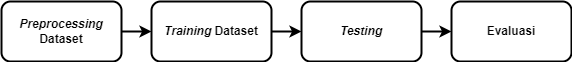
\includegraphics[scale=0.75]{gambar/metodologi.png}
  % Keterangan gambar yang diinputkan
  \caption{Diagram Desain Sistem}
  % Label referensi dari gambar yang diinputkan
  \label{fig:DiagramMetodologi}
\end{figure}

\subsection{\emph{Preprocessing} Dataset}

Pada tahap ini, dataset yang sudah ada akan melalui beberapa proses terlebih dahulu sebelum memasuki tahap \emph{training}. Beberapa proses tersebut diantaranya adalah membersihkan dataset, augmentasi gambar, dan pembagian dataset. Hal tersebut dilakukan agar proses \emph{training} menjadi lebih optimal.

\subsection{\emph{Training} Dataset}

Dataset yang sudah diproses pada tahap \emph{preprocessing} akan dilakukan \emph{training} menggunakan metode CNN. Hasil dari tahap ini berupa model CNN yang dapat melakukan reidentifikasi kendaraan.

\subsection{\emph{Testing}}

Testing dilakukan untuk menguji model yang sudah dibuat. Apabila hasil kurang sesuai, maka akan dilakukan training lagi untuk mendapatkan model yang lebih baik dan hasil testing bisa lebih akurat. Testing akan menggunakan citra baru atau citra yang belum digunakan dalam tahap training. Hal ini untuk benar-benar menguji keberhasilan model yang sudah dibuat.

\subsection{Evaluasi}

Pada tahap ini, seluruh proses penelitian yang sudah dilakukan akan dievaluasi. Proses evaluasi juga meliputi penarikan kesimpulan dan menentukan kelayakan model dalam melakukan reidentisikasi kendaraan.

\section{Data dan peralatan yang digunakan}

\begin{enumerate}[label=(\alph*)]
  \item Dataset
        \begin{figure} [ht] \centering
          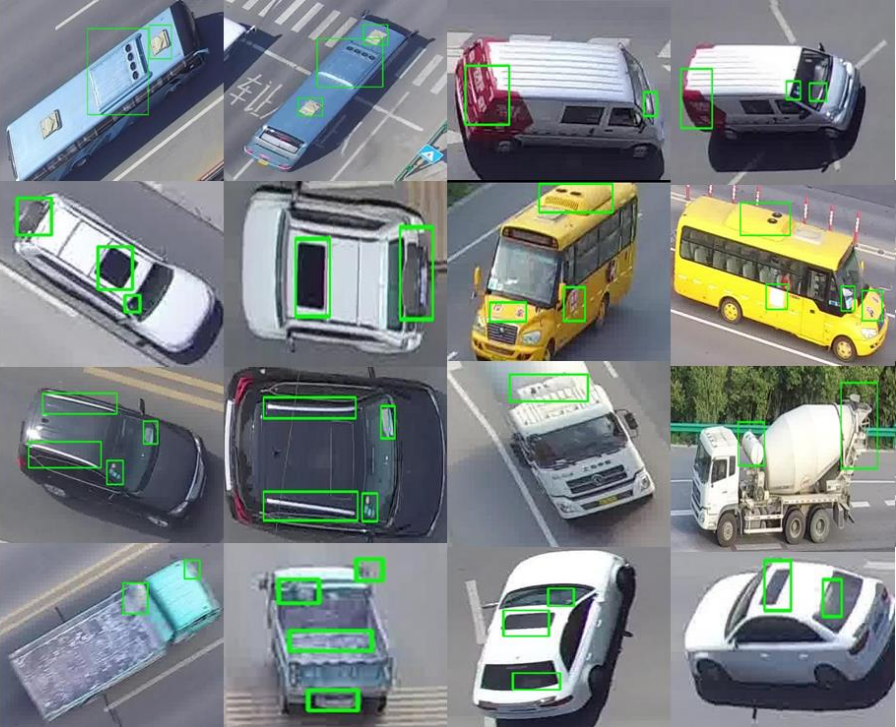
\includegraphics[scale=0.4]{gambar/VRAI-dataset.png}
          \caption{Sampel Citra yang Ada pada Dataset VRAI}
          \label{fig:VRAIDatset}
        \end{figure}

        Dataset yang digunakan pada penelitian ini merupakan dataset yang diambil dari repositori publik github milik JiaoBL1234 \cite*{VRAIDatasetGithub}. Berdasarkan paper yang berjudul ”Vehicle Re-identification in Aerial Imagery: Dataset and Approach”, Peng Wang et al membuat dataset untuk reidentifikasi kendaraan dengan mengaplikasikan UAV sebagai alat pengambil citra. Dataset tersebut diberi nama Vehicle Re-identification for Aerial Image (VRAI). Dataset VRAI terdiri dari 137.613 gambar dari 13.022 sampel kendaraan. Gambar dari setiap sampel kendaraan ditangkap oleh kamera dari dua UAV bermerek DJI di lokasi yang berbeda, dengan berbagai sudut pandang dan ketinggian terbang (15m hingga 80m) \cite{Wang2019vehicle}.

        \newpage

  \item Laptop

        Laptop digunakan untuk pengerjaan penelitian ini, mulai dari \emph{Preprocessing} Dataset, \emph{Training} Dataset, \emph{Testing}, maupun penyusunan laporan. Laptop yang digunakan adalah laptop pribadi milik penulis. Adapun merek dari laptop yang digunakan adalah Lenovo Legion 5 tipe 15ARH05H dengan spesifikasi sebagai berikut:
        \begin{longtable}{|c|c|c|}
          \caption{Spesifikasi Laptop}
          \label{tb:spesifikasilaptop}                    \\
          \hline
          % \rowcolor[HTML]{C0C0C0}
          \textbf{Tipe}      & \textbf{Detail}            \\
          \hline
          \textit{Processor} & AMD Ryzen 7 4800H          \\
          Memory             & 16 GB                      \\
          Storage            & SSD 1TB                    \\
          Graphic Card       & NVIDIA GeForce GTX 1660 Ti \\
          Operating System   & Windows 11                 \\
          \hline
        \end{longtable}
  \item Google Colaboratory

        Google Colaboratory atau biasa disebut "Google Colab" adalah produk dari Google Research. Google Colab memungkinkan siapa saja untuk menulis dan mengeksekusi kode python arbitrer melalui browser, dan sangat cocok untuk pembelajaran mesin, analisis data, dan pendidikan \cite{GoogleColab}. Pada penelitian ini, Google Colab digunakan sebagai \emph{platform} untuk menulis semua kode program dan juga untuk melakukan penelitian khususnya dalam preprocessing data, training data, dan testing data.
\end{enumerate}

\newpage

\section{Urutan pelaksanaan penelitian}

Penelitian ini akan dilaksanakan selama 16 minggu. Urutan pelaksanaan penelitian ini dapat dilihat pada tabel \ref{tb:TimelinePenelitian}.
% Ubah tabel berikut sesuai dengan isi dari rencana kerja
\newcommand{\w}{}
\newcommand{\G}{\cellcolor{gray}}
\begin{table}[h!]
  \caption{\label{tb:TimelinePenelitian}\emph{Timeline} Penelitian}
  \begin{tabular}{|p{3.5cm}|c|c|c|c|c|c|c|c|c|c|c|c|c|c|c|c|}

    \hline
    \multirow{2}{*}{Kegiatan} & \multicolumn{16}{|c|}{Minggu}                                                                       \\
    \cline{2-17}              &
    1                         & 2                             & 3  & 4  & 5  & 6  & 7  & 8  & 9  & 10 & 11 & 12 & 13 & 14 & 15 & 16 \\
    \hline

    % Gunakan \G untuk mengisi sel dan \w untuk mengosongkan sel
    Studi Literatur           &
    \G                        & \G                            & \w & \w & \w & \w & \w & \w & \w & \w & \w & \w & \w & \w & \w & \w \\
    \hline

    Preprocessing Data        &
    \w                        & \w                            & \G & \G & \G & \w & \w & \w & \w & \w & \w & \w & \w & \w & \w & \w \\
    \hline

    Training data             &
    \w                        & \w                            & \w & \w & \G & \G & \G & \G & \G & \G & \G & \G & \G & \w & \w & \w \\
    \hline

    Testing                   &
    \w                        & \w                            & \w & \w & \w & \w & \w & \w & \w & \w & \G & \G & \G & \w & \w & \w \\
    \hline

    Evaluasi                  &
    \w                        & \w                            & \w & \w & \w & \w & \w & \w & \w & \w & \w & \w & \w & \G & \G & \w \\
    \hline

    Pembuatan Laporan         &
    \G                        & \G                            & \G & \G & \G & \G & \G & \G & \G & \G & \G & \G & \G & \G & \G & \G \\
    \hline
  \end{tabular}
\end{table}

\newpage
\cleardoublepage

% Konten hasil
\chapter{HASIL DAN PEMBAHASAN}

\section{Hasil yang Diharapkan dari Penelitian}

Hasil yang diharapkan dari penelitian ini adalah model reidentifikasi yang dibuat pada penelitian ini memiliki nilai akurasi yang lebih tinggi atau setidaknya menyamai penelitian sebelumnya yang menggunakan dataset CCTV. Penulis juga berharap penelitian mengenai reidentifikasi mobil dengan memanfaatkan UAV akan lebih banyak dipelajari oleh para peneliti.

\section{Hasil Pendahuluan}

Sejauh ini penulis telah menentukan dataset yang akan digunakan dalam penelitian ini. Selain itu, penulis juga sudah mempelajari mengenai \emph{Convolutional Neural Network} (CNN) dan juga membaca penelitian-penelitian terkait sistem reidentifikasi kendaraan berbasis \emph{Convolutional Neural Network} (CNN). Penulis juga sudah mencoba melakukan \emph{training} dataset menggunakan model arsitektur ResNet-50 yang menghasilkan suatu model \emph{deep learning} yang dapat melakukan klasifikasi bunga. Saat ini, penulis sedang melakukan tahap \emph{preprocessing} dataset. Tahap \emph{preprocessing} yang sedang dilakukan yaitu \emph{splitting} dataset. Dalam proses \emph{splitting}, citra-citra pada dataset akan dibagi ke dalam \emph{folder-folder} yang sesuai sehingga akan memudahkan saat proses \emph{training}.

\newpage
\cleardoublepage

% Konten penutup
\chapter{PENUTUP}

\section{Kesimpulan}

Hasil yang diharapkan dari penelitian ini adalah model reidentifikasi yang dibuat pada penelitian ini memiliki nilai akurasi yang lebih tinggi atau setidaknya menyamai penelitian sebelumnya yang menggunakan dataset CCTV. Penulis juga berharap penelitian mengenai reidentifikasi mobil dengan memanfaatkan UAV akan lebih banyak dipelajari oleh para peneliti.

\section{Saran}

Sejauh ini penulis telah menentukan dataset yang akan digunakan dalam penelitian ini. Selain itu, penulis juga sudah mempelajari mengenai \emph{Convolutional Neural Network} (CNN) dan juga membaca penelitian-penelitian terkait sistem reidentifikasi kendaraan berbasis \emph{Convolutional Neural Network} (CNN). Penulis juga sudah mencoba melakukan \emph{training} dataset menggunakan model arsitektur ResNet-50 yang menghasilkan suatu model \emph{deep learning} yang dapat melakukan klasifikasi bunga. Saat ini, penulis sedang melakukan tahap \emph{preprocessing} dataset. Tahap \emph{preprocessing} yang sedang dilakukan yaitu \emph{splitting} dataset. Dalam proses \emph{splitting}, citra-citra pada dataset akan dibagi ke dalam \emph{folder-folder} yang sesuai sehingga akan memudahkan saat proses \emph{training}.

\newpage
\cleardoublepage

% Daftar pustaka
\chapter*{DAFTAR PUSTAKA}
\addcontentsline{toc}{chapter}{DAFTAR PUSTAKA}
\renewcommand\refname{}
\vspace{2ex}
\renewcommand{\bibname}{}
\begingroup
\def\chapter*#1{}
\printbibliography
\endgroup


\end{document}
